\chapter{Versioned Interoperability: MCP, A2A, and Protocol Boundaries}\label{ch:C19}

MCP's 2026-07-28 specification replaces the legacy initialization handshake with self-contained per-request version and capability declarations~\cite{mcp2026spec,mcp2026schema}. A2A addresses a different boundary: delegated work represented through messages, tasks, and artifacts~\cite{a2a2026task}. Neither protocol by itself establishes sufficient agent context, permission to execute an effect, or correctness of a returned artifact.

\section{Protocol compatibility is not agent competence}\label{sec:C19:scope}
An interoperability protocol standardizes messages and declared behavior across process or organizational boundaries. It can make tools discoverable, data addressable, and delegated work trackable. It does not determine whether an agent chooses the right capability, constructs a correct plan, or interprets evidence appropriately. A protocol-conformant system can execute a perfectly well-formed but irrelevant or unauthorized operation if the surrounding application grants it that authority.

MCP and A2A address different boundaries. MCP connects an application host and its clients to servers exposing context and capabilities. A2A represents interactions with a remote agent through messages, tasks, artifacts, and declared capabilities~\cite{mcp2026spec,cumb2026a2aspec101}. A tool server can wrap sophisticated computation, and a remote agent can internally use many tools. The distinction is the contract exposed to the caller, not an ontological test of whether the remote implementation is intelligent.

The literature and implementation review for this chapter is current through 29 October 2026. The current MCP revision identified in the official versioning documentation is 2026-07-28~\cite{mcp2026versioning}. The versioning policy permits backwards-compatible changes while a revision is current, so a dated specification URL alone does not freeze every document; the inspected schema commit is recorded separately. Earlier handshake-based revisions remain historically important, but their session and initialization assumptions must not be presented as the current core protocol. A2A's task lifecycle is anchored to the v1.0.1 repository snapshot~\cite{a2a2026task}; ancillary documentation using a moving ``latest'' URL remains a reproducibility limitation unless archived or pinned independently.

The application must map protocol identities to its own semantic identities. A JSON-RPC request identifier correlates a request and response. It is not automatically a durable task identifier, a user session, or an idempotency key for an external effect. Similarly, a remote agent's declared name is not proof of its authority. Confusing these roles can produce duplicate work, cross-session state mixing, or misplaced trust while every message still validates against a schema.

For technical comparison, define interoperability at several levels: transport connectivity, message-schema compatibility, feature negotiation, semantic agreement about state transitions, authority propagation, and reliable recovery. Passing a connectivity test establishes only the first levels. A useful conformance report should identify which levels were exercised and which remain assumptions. The analysis below separates the current normative message facts from the systems deductions that follow when those messages carry long-running agent work.


% SCIENTIFIC_FIGURE_C19
Figure~\ref{fig:C19:overview} distinguishes request correlation, task lifecycle, and conversational context; none of these identifiers establishes current dispatch authority.
\begin{figure}[!htbp]
\centering
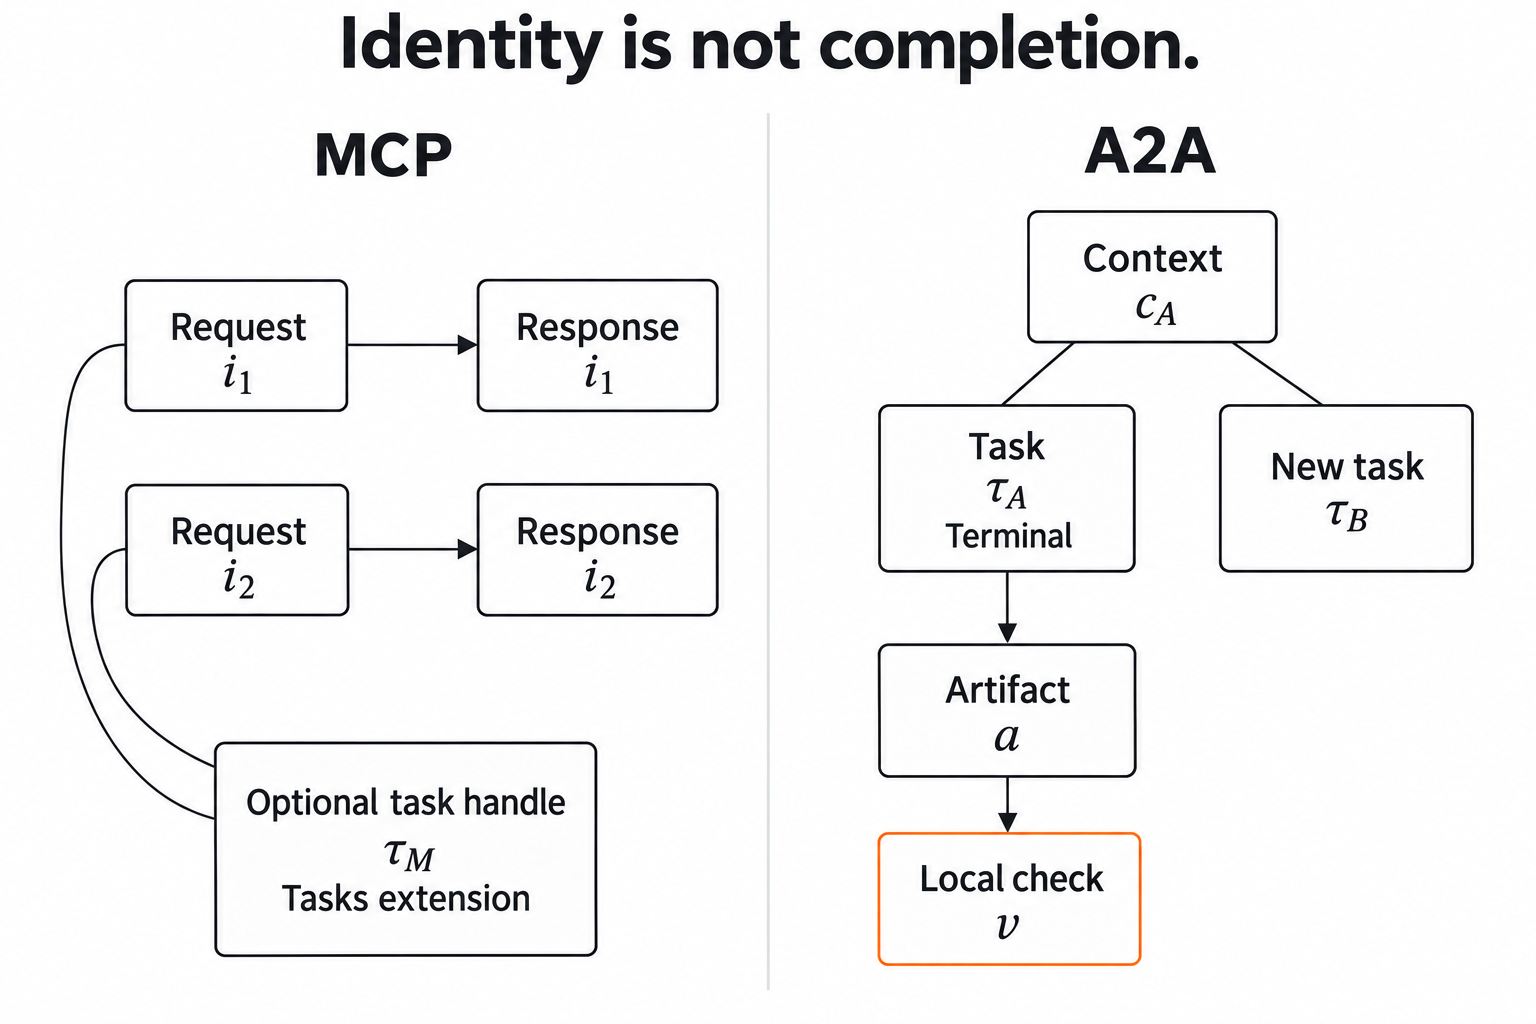
\includegraphics[width=\linewidth]{book/figures/assets/F19review.png}
\caption{Protocol identifiers bind different objects. MCP RPC identifiers correlate individual exchanges; an optional Tasks-extension handle can relate requests to durable work. A2A context identifiers group interactions, while task identifiers bind units of work. A terminal task is not restarted; a later follow-up can create a new task in the same context. Returned artifacts still need local validation. No automatic cross-protocol identity or authority mapping is implied.}
\label{fig:C19:overview}
\end{figure}

\section{Modern MCP declares versions on every request}\label{sec:C19:versioning}
MCP 2026-07-28 uses per-request version and capability metadata, without a negotiation handshake. The server accepts or rejects each request independently. Servers implement \path{server/discover}; clients may call it to obtain supported versions, capabilities, and identity, but may also send another request directly and handle an unsupported-version error~\cite{mcp2026compat,mcp2026discover}. This is the current behavior, not a renamed form of the legacy initialization sequence.

The base protocol requires the protocol-version and client-capabilities fields in request \path{_meta}; client identity is recommended but not universally required~\cite{mcp2026base}. The tool page's prefatory example note groups identity with required metadata, whereas the base requirements and \texttt{RequestMetaObject} make it optional. Requiredness here follows those explicit base and schema definitions~\cite{mcp2026tools,mcp2026schema}. A discovery request can be described as a typed record without conflating its wire encoding with its semantic identities. Let $\mathcal Q,\mathcal I,\mathcal M$, and $\mathcal P$ be the admissible RPC versions, correlation identifiers, methods, and parameter records. A constructed request is
\begin{equation}
\begin{aligned}
 r_d&=(\rho_2,i_d,m_d,p_d)
       \in\mathcal Q\times\mathcal I\times\mathcal M\times\mathcal P,\\
 p_d&=\langle\mu_d\rangle,\qquad
 \mu_d=(v_\star,C_d),\qquad C_d=\varnothing.
\end{aligned}
\label{eq:C19:discovery_request_record}
\end{equation}
The first four coordinates encode the \path{jsonrpc}, \path{id}, \path{method}, and \path{params} fields. The constant $\rho_2$ denotes JSON-RPC 2.0, $i_d$ an arbitrary request-correlation identifier, and $m_d$ the \path{server/discover} method. Inside the parameter record, $\mu_d$ encodes \path{_meta}; $v_\star$ is the 2026-07-28 revision carried by \path{io.modelcontextprotocol/protocolVersion}, and $C_d$ is the capability-declaration map carried by \path{io.modelcontextprotocol/clientCapabilities}. The empty map declares no client capabilities. These coordinates do not identify a durable task, conversational session, or external-effect key.

Equation~\ref{eq:C19:discovery_request_record} is a constructed schema-level record, not a trace from a tested server or a complete JSON serialization. On Streamable HTTP, the declared version is also represented in the protocol-version header under the transport's rules. A mismatch must be treated according to that binding rather than silently guessing which version the peer intended.

The same revision makes result interpretation explicit through \texttt{resultType}. Core values distinguish \texttt{complete} from \path{input_required}; a value unrecognized by both the core and agreed extensions is invalid, while an absent field from an earlier server is treated as complete for compatibility~\cite{mcp2026base}. An input-required result is neither a completed tool effect nor a generic transport error. It can carry input requests, opaque continuation state, or both; continuation state alone need not mean that a user form is missing. A resubmission follows that continuation contract, uses a new RPC correlation identifier, and preserves the application operation identity where applicable. The continuation token is not itself a grant or proof of effect completion. This spelling and message role also differ from A2A's interrupted task state: translating between the protocols requires a semantic mapping, not replacement of one status string by another.

An unsupported-version response lists supported versions, allowing the client to retry with a mutually supported choice or surface incompatibility~\cite{mcp2026compat}. The retry should preserve the application operation's identity while respecting that a protocol retry and an effect retry are different concepts. A rejected version normally precedes application execution, but clients should not generalize that ordering to arbitrary transport failures or tool timeouts.

Self-contained requests reduce reliance on connection-local negotiation state. They do not mean that the server cannot maintain application data. Persistent state must be referenced explicitly rather than inferred from a shared socket or process. This supports multiplexing unrelated tasks while making the application responsible for its own session and authorization identifiers. Reusing a connection does not create a shared conversational memory contract.

Legacy revisions through 2025-11-25 establish a session through initialization. A dual-era implementation can support both modern and legacy behavior, using the transport-specific fallback rules~\cite{mcp2026compat}. A recognized modern error should not be mistaken for evidence that the peer is legacy. An indiscriminate fallback can hide a real version or capability error and accidentally select weaker semantics. Compatibility testing should therefore exercise explicit modern rejection, genuine legacy behavior, and a peer supporting both eras.


\section{Tools resources prompts and skills remain distinct}\label{sec:C19:primitives}
MCP exposes several kinds of objects whose roles should remain separate. Tools are invocable capabilities with schemas; resources expose addressable context; prompts provide reusable interaction templates~\cite{mcp2026spec}. A host decides how those objects enter the model's working view. The protocol does not specify a universal context-selection, memory-consolidation, or reasoning policy. A shared transport therefore does not make every object an instruction or every server a memory system.

The current tool interface separates listing from invocation through \path{tools/list} and \path{tools/call}. Available tools can depend on request authorization, and descriptions and schemas guide the caller~\cite{mcp2026tools}. The host still needs grounding, argument validation, and an authority check before effects. A tool annotation is not a substitute for an enforced permission boundary. Chapter~\ref{ch:C18} analyzes these application-level contracts.

Resources have URI identities and can be listed, read, or described through templates~\cite{mcp2026resources}. A resource URI is a reference in the server's namespace, not necessarily a local filesystem path accessible to the client. The host should preserve the server and version context when storing or citing retrieved content. If a resource later changes, a previous citation requires a content snapshot or version reference to remain reproducible. A stable URI alone does not imply immutable evidence.

A skill is procedural knowledge packaged for selective use, as developed in Chapter~\ref{ch:C15}. It may be delivered through a protocol extension or represented using resources, prompts, and tools, but those representations do not collapse its meaning into the underlying primitive. The Agent Skills specification concerns the skill artifact; MCP concerns exchange and invocation; the model policy decides applicability. A skill can instruct the use of a tool without having authority to grant access to it~\cite{agentskills2026spec}.

This separation has a concrete security consequence. A retrieved resource can contain adversarial text that asks the agent to change its goal. The host should label it as untrusted evidence rather than promote it to a privileged instruction. A prompt template can be selected by an authorized user while still containing external fields that require careful interpolation. A tool result can contain both structured data and explanatory prose with different trust properties. These distinctions must survive serialization and compaction.

The proposed implementation stores a typed provenance envelope for every imported object: server identity, object kind, object identifier, schema or content version, access scope, and insertion role. A context assembler then decides what is visible without losing those labels. This is an application design, not a protocol guarantee. It makes cross-layer errors observable when the same bytes are later retrieved as memory or passed to another agent.


\section{Transport statelessness and explicit durable work}\label{sec:C19:transport}
The 2026-07-28 Streamable HTTP binding changed earlier behavior by removing the GET stream endpoint and protocol-level sessions~\cite{mcp2026http}. A description of the old transport that assumes those features remain current is technically wrong. Streaming and long-lived work must be interpreted through the current binding and per-request declared features rather than inherited from a historical tutorial. Transport connections remain implementation resources, not semantic user sessions.

The base protocol's statelessness means that requests carry the information required to interpret them, with longer-lived application state referenced explicitly~\cite{mcp2026base}. A server can still operate on a database, a file collection, or an ongoing job. The critical rule is that the server should not infer user or task continuity from connection reuse. A reconnect should not require the client to recreate an implicit conversational state hidden inside the old transport.

The Tasks extension supports long-running operations through explicit durable handles and subsequent status or result access~\cite{mcp2026tasks}. Extension support is not assumed for every core endpoint. The returned task includes a retention lifetime and polling interval; a durable handle is not a promise of indefinite result availability. Cancellation is cooperative and can still end in a different terminal state~\cite{mcp2026tasks}. The client must distinguish a synchronous complete result from a durable pending operation and preserve the handle in its task state. Dropping the handle during compaction can make the agent lose track of work that continues remotely. Creating a new call in response can duplicate the operation rather than resume it.

A proposed application state machine records pending, awaiting input, completed, failed, canceled, and outcome-unknown states as appropriate to the negotiated feature. The exact protocol states should follow the cited extension; the application can refine them to track external effects. Cancellation of a request, cancellation of remote work, and compensation of an already committed effect are distinct operations. A successful cancel response should be interpreted within the remote service's stated semantics.

Progress notifications are useful for liveness monitoring but do not prove successful task completion. A stream can stop because the network failed while the remote work continues. A host should retain explicit operation identifiers and use a status or reconciliation path when available. The same reasoning applies to retries after a timeout: a self-contained request improves routing and interpretation, but does not by itself make the requested effect idempotent.

The engineering benefit of the modern boundary is that session meaning becomes explicit. The cost is that applications cannot rely on an old initialization handshake to carry hidden task continuity. Durable agent state must record handles, versions, authority, and receipts independently of the socket. This aligns the protocol layer with the session contracts in Chapter~\ref{ch:C13} and makes failure recovery a testable application responsibility.


\section{Authorization is separate from declared identity}\label{sec:C19:authorization}
MCP's HTTP authorization specification distinguishes client, protected resource server, resource owner, and authorization server roles. Authorization is optional at the protocol-implementation level; HTTP implementations that support it SHOULD conform to the cited framework, while stdio implementations SHOULD instead obtain credentials from their environment~\cite{mcp2026auth}. A server being reachable does not imply that every capability is authorized, and a client being authenticated does not imply that every requested effect is within the user's task scope.

The current specification uses protected-resource and authorization-server discovery mechanisms and defined registration options~\cite{mcp2026auth}. These are protocol and credential contracts, not a complete application policy. An access token can permit a broad API scope while the current user request authorizes only a narrow task. A local monitor may need to enforce the narrower boundary even when the remote service accepts the credential.

The protocol's client and server information fields are self-reported metadata rather than cryptographic proof of identity~\cite{mcp2026discover}. Applications should not treat a familiar display name or version string as authorization evidence. Trust should derive from the configured endpoint, transport authentication, credential validation, and applicable policy. This is particularly important for discovery catalogs that combine many servers with similar tool names.

Delegation adds another question: whose authority is being exercised? A host can authenticate to a tool server using its own credential while acting on behalf of a user. A remote agent can request a capability that the original user never intended to delegate. The application should preserve the principal and scope through each hop, avoiding silent expansion when a worker or skill is loaded. Protocol compatibility makes the message exchange possible; it does not decide the appropriate delegation policy.

Credential exposure should not be treated as ordinary memory. The model generally needs a capability reference and allowed scope, not a plaintext token in its context. If a token or secret enters a tool result, subsequent summaries and indexes can spread it beyond its intended lifetime. A secure wrapper can keep credentials outside the model-visible evidence packet while recording which credential scope admitted an effect. The exact storage and redaction mechanism remains application-specific.

A proposed authorization test matrix includes correct credentials with excessive task scope, stale authorization after a user correction, catalog changes under different principals, and a reconnect that interleaves unrelated users. Measure both unauthorized acceptance and false rejection of legitimate work. A system that blocks every call is not a useful agent, while one that completes every task with broad credentials has not demonstrated least-privilege operation.


\section{A2A tasks artifacts and delegated autonomy}\label{sec:C19:a2a}
A2A allows a remote agent to respond with a self-contained message or initiate stateful work represented as a task. Its lifecycle distinguishes interrupted states, such as \texttt{input-required} or \texttt{auth-required}, from terminal outcomes. A context identifier can group multiple interactions, while a task identifier refers to a particular unit of work~\cite{a2a2026task}. These identifiers should not be mapped automatically to the model's active context window or to one transport connection.

Terminal tasks do not restart. A refinement creates new work within the related context and can reference the earlier task~\cite{a2a2026task}. Consequently, client artifact acceptance and mutation lineage must survive beyond the producing task's terminal status. Reusing the old task identifier as a mutable revision slot would obscure which input produced which artifact. Continuity belongs to the explicit context and client-managed lineage, while terminal task identity preserves the completed unit of work.

A2A v1.0.1 also distinguishes idempotency by operation. Reads are naturally idempotent, message submission MAY use the message identifier for duplicate detection, and task cancellation is idempotent~\cite{cumb2026a2aspec101}. Thus a repeated message identifier is not a universal delivery guarantee, and idempotent cancellation does not establish rollback of a previously committed effect. The client must record which remote deduplication contract was actually promised.

Discovery uses an Agent Card describing offered capabilities, endpoints, input and output modes, and security-related information~\cite{cumb2026a2adiscovery101}. The card supports selection of a suitable remote agent; it does not prove the agent's competence. A skill description in the card is an advertised capability, not necessarily a portable executable skill package. The caller still needs task validation, evidence handling, and a policy for trusting returned artifacts.

Delegating a task differs from invoking a narrow tool because the remote agent can choose internal methods and produce intermediate work. The caller may observe only status and artifacts rather than every internal action. This can be useful for modularity and privacy, but it changes verification. A completed task state is a protocol statement from the remote service, not independent proof that the original user's success predicate was met.

Artifacts should preserve provenance, version, and a relation to the task. A document returned by a remote researcher can contain supported claims, unsupported synthesis, or stale citations. An execution artifact can be syntactically valid while violating a local constraint unknown to the remote agent. The delegation request should therefore include the relevant obligations and authority, and the caller should validate the artifact against them before publication or further effects.

Parallel follow-ups create a state-ownership problem. Several tasks can share a context identifier while working on different branches of an objective. A late artifact from one branch should not silently overwrite a newer accepted artifact from another. The application needs version and acceptance rules beyond the protocol's ability to transport updates. Similarly, a request for more information should suspend or qualify dependent work rather than being ignored while the caller assumes progress.

A proposed delegation contract contains goal, completion predicate, budget, permitted effects, evidence requirements, and expected artifact schema. It allows the remote agent flexibility within those constraints. A callback or streaming update can report progress, while final acceptance remains a separate local decision. This distinguishes negotiated autonomy from unrestricted trust and connects protocol design to the orchestration analysis in Chapter~\ref{ch:C21}.


\section{A concrete cross-protocol execution trace}\label{sec:C19:trace}
Artifact transfer needs an explicit trust boundary. An A2A artifact identifier belongs to the producing task's namespace; an MCP resource identifier belongs to the serving endpoint's namespace. Resolving one into the other is an application mapping, not an equality implied by the identifier strings. A content digest can detect a changed payload but cannot establish the producer's authority or the truth of its claims. Preserve the producing task, source version, content type, and verification status when constructing the resource representation. The consumer should distinguish an agent's inference from evidence that the remote agent actually observed. Otherwise a technically correct transfer can launder a speculative conclusion into an apparently authoritative tool result.

An interrupted task also needs a scope-preserving continuation rule. Suppose a remote agent requests authorization for one operation and later resumes with changed arguments. Reusing the earlier approval solely because the task identifier is unchanged can authorize a different effect. A proposed application contract binds a grant to the relevant argument digest, resource scope, authority epoch, and expiry; a changed material precondition requires revalidation. This is an authority requirement derived from the execution model, not a claim that every A2A implementation enforces that binding. Protocol progress and user authorization are separate state machines, even when one user interface displays them together.

Consider a constructed workflow in which a coordinator delegates a research task to a remote agent and later uses a tool server to retrieve a source record. The A2A request identifies the objective, current constraints, and expected evidence artifact. The remote service returns a task handle or a direct message according to its supported interaction. The coordinator records the handle in durable task state rather than relying on an open stream to remember it.

When evidence requires a tool server, the coordinator's MCP client sends a request carrying the current protocol version and client capabilities. It may first use discovery, then list the authorized tools and obtain the selected schema. Before invoking the tool, the host validates arguments and task authority. The server's response becomes a typed observation with server and resource identity. It does not become a new user instruction merely because it was returned through a trusted transport.

Suppose the research task returns a completed artifact while one cited resource has changed. The coordinator should validate the cited version or preserve the captured passage, then decide whether the artifact satisfies the requested evidence standard. If the artifact proposes publication but the delegation allowed only preparation, local authority remains binding. A2A task completion and MCP tool success do not jointly imply permission to publish.

Now interrupt the network after a tool operation may have committed but before the coordinator receives the result. Reconnecting with the correct protocol metadata does not resolve the effect. The application needs an explicit operation identifier, remote status query, or reconciliation procedure. If no such mechanism exists, it should retain an outcome-unknown state. Reissuing the same semantic request with a new JSON-RPC identifier can duplicate work unless the tool supplies an independent idempotency contract.

This trace is original synthesis, not a tested integration or a claim that every SDK implements these steps. It identifies the records a correct implementation would need: delegation identifier, task/context relation, protocol versions, catalog/schema digest, authorization version, effect identifier, response receipt, and artifact acceptance decision. These records support causal diagnosis if the final output is wrong.

The most informative interoperability experiment would replay this workflow with independent client and server implementations, controlled delays, credential changes, and a mixed modern/legacy MCP environment. A successful result would support the tested semantic contract, not merely that two programs exchanged JSON. A failed result should identify whether the mismatch concerned version negotiation, capability declaration, effect semantics, or the meaning of task completion.

The normative implementation anchor is the versioned TypeScript schema. At the inspected July 28 commit, \texttt{RequestMetaObject} requires the protocol-version and client-capabilities members while declaring client information optional. \texttt{DiscoverRequest} fixes the discovery method, and \texttt{CallToolRequest} binds the tool-call method to its parameter structure~\cite{mcp2026schema}. These definitions are stronger implementation references than copying an old SDK example and assuming it speaks the current protocol. They describe message shape; they are not an executed conformance test of any client library.

A concrete negative test removes only the capabilities member from the illustrative request while preserving valid JSON and a recognized version. A second test keeps the capabilities member but changes the HTTP version header so it disagrees with the body. A third requests an unsupported protocol version while keeping body and header equal. These cases should not collapse into one generic retry: malformed metadata, inconsistent transport declaration, and unsupported version are different failures. Their distinction matters because only some errors justify selecting a different protocol version.

An application can generate clients from schema definitions and still mishandle those outcomes. It might cache a successful discovery response under one credential and reuse the catalog under another. It might regard an optional identity string as a trusted principal. It might strip required metadata when forwarding a request to a worker. These are integration failures above the type definition. Test the complete forwarding path with different principals and concurrent tasks rather than validating only an isolated client serializer.

For long-running operations, retain two kinds of correlation. The protocol request identifier tracks a particular exchange, while an explicit application or extension handle tracks durable work. After a reconnect, a new exchange can refer to the same durable task. If the implementation uses request identity as the only operation identity, it can either duplicate work on retry or incorrectly suppress a legitimate new request. A reference fixture should model both identities and assert which one is stable across network retries.

The same distinction supports audit of delegated research. The coordinator can record that a remote task completed and that an artifact was received, while separately recording whether the artifact passed evidence validation. This avoids turning transport success into scientific acceptance. It also allows the coordinator to reject one artifact without falsely marking the remote operation as never completed. Protocol state, task state, and epistemic status remain separate even when the user interface displays one compact progress indicator.


\section{Conformance performance and residual uncertainty}\label{sec:C19:evaluation}
Protocol evaluation should separate schema conformance from application correctness. Conformance tests can validate required metadata, unsupported versions, capability errors, pagination, and response correlation. They can inspect whether the current modern request model is implemented rather than a historical initialization flow. They cannot establish that an agent's chosen action is useful or that a returned research artifact is scientifically sound.

Use a version matrix with modern-only, legacy-only, and dual-era MCP peers. Include missing required metadata, declared but unsupported capabilities, an unknown version, and a recognized modern rejection. Test whether fallback follows the binding's rules instead of treating every error as a reason to initialize a legacy session. Preserve exact specification and SDK revisions in the result. A package release number alone is insufficient when examples or generated schemas change independently.

For A2A, test direct messages, stateful tasks, interrupted work, terminal outcomes, and artifact updates. Include delayed and duplicated updates, failed streams, and concurrent follow-ups. Check that the application preserves task ownership and does not interpret a progress event as completion. Independently verify a sample of final artifacts against the requested predicate. Protocol-level terminal status and task-level validity should remain separate metrics.

Performance accounting includes discovery, schema transfer, serialization, credential flows, network latency, polling or streaming overhead, model decisions, and remote work. Compare warm and cold operation, and identify which metadata is cacheable under which principal. A cached catalog can reduce overhead while becoming stale after a permission or tool change. Latency gains should therefore be reported alongside freshness and correctness behavior.

The official MCP architecture documentation identifies an additional current-version change: sampling and some prior utilities are deprecated in the 2026-07-28 era, and change notifications are delivered through opt-in subscriptions~\cite{mcp2026architecture}. Implementations and surveys should not infer present support from an older tutorial. Deprecation also differs from immediate removal; the exact feature lifecycle must be checked before asserting that a capability is unavailable.

No runtime conformance or cross-protocol benchmark has been executed for this chapter. The normative facts come from official specifications inspected at the cutoff; the execution trace, failure analysis, and test design are explicitly deductions and proposals. The main technical conclusion is bounded: interoperable messages make component composition possible, while durable state, authority, evidence quality, and verified outcomes remain contracts of the complete agent system. Those contracts determine whether interoperability improves reliable autonomy.

